\documentclass{article}
\usepackage{graphicx} % Required for inserting images

\title{\textbf{Labwork 3: Hello, CUDA!}}
\author{Nguyen Thanh Binh}
\date{\today}

\usepackage{hyperref}
\hypersetup{
    colorlinks=true,
    linkcolor=blue,
    filecolor=magenta,      
    urlcolor=cyan,
    pdftitle={Overleaf Example},
    pdfpagemode=FullScreen,
    }

\begin{document}

\maketitle

\section{Loading image:}

For this section, we will use \texttt{matplotlib.pyplot} to load an image with the \texttt{imread} function. This function allows an input of a png file, which has four channels, or an jpg file with three channels. For the data type, it will be \texttt{NDArray}

\begin{verbatim}
from numba import cuda
import math
import matplotlib.pyplot as plt
import numpy as np
import matplotlib.image as mping
\end{verbatim}

\begin{verbatim}
image = mping.imread("your file directory")
plt.imshow(image)
\end{verbatim}

\begin{figure}
    \centering
    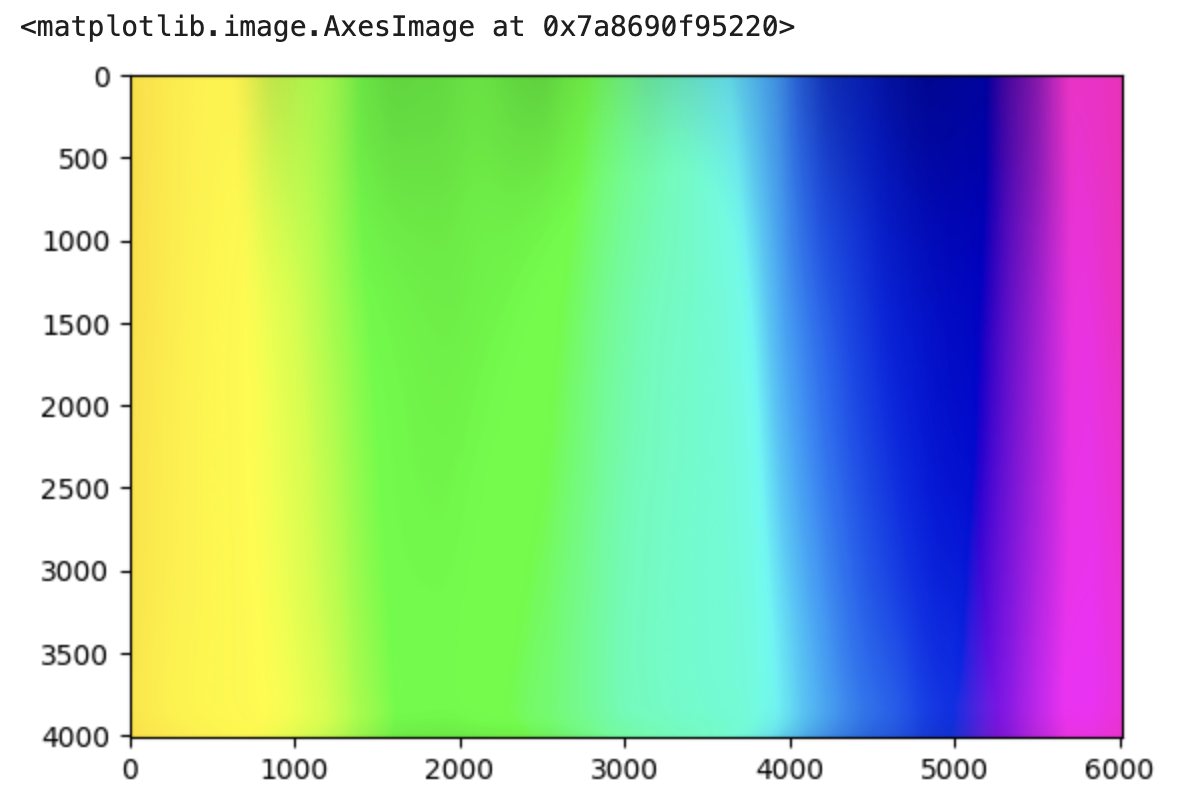
\includegraphics[width=1\linewidth]{sample.png}
    \caption{Image loaded using \texttt{matplotlib.pyplot.imread}}
    \label{fig:placeholder}
\end{figure}

\section{Grayscaling:}

As the title suggests, we will use CUDA only, which is \texttt{numba.cuda} package, specifically. 

 We begin by setting up our host and feeding device with data:

\begin{verbatim}
# Input to device
d_host = cuda.to_device(img)
# Memory allocation for output values
d_img = cuda.device_array_like(img)
\end{verbatim}

Once the setup is complete, we will create a kernel for the device to process:

\begin{verbatim}
@cuda.jit
def grayscale(src, dst):
# where are we in the input?
  tidx = cuda.threadIdx.x + cuda.blockIdx.x * cuda.blockDim.x
  g = np.uint8((src[tidx, 0] + src[tidx, 1] + src[tidx, 2]) / 3)
  dst[tidx, 0] = dst[tidx, 1] = dst[tidx, 2] = g
\end{verbatim}

After we have finished creating kernels, it is time to launch the kernel. In this case to grayscale image, we need to define block size for processing. 

\begin{verbatim}
# Get length for each dimension
imageH = image.shape[0]
imageW = image.shape[1]
imageDim = image.shape[2]

pixelcnt = imageH * imageW
blockSize = 64
gridSize = pixelcnt // blockSize

grayscale[gridSize,blockSize](d_host,d_image)
\end{verbatim}

To get results from the device: 
\begin{verbatim}
    result = d_image.copy_to_host()
\end{verbatim}

This function will copy the result from the device to host. 

\begin{figure}
    \centering
    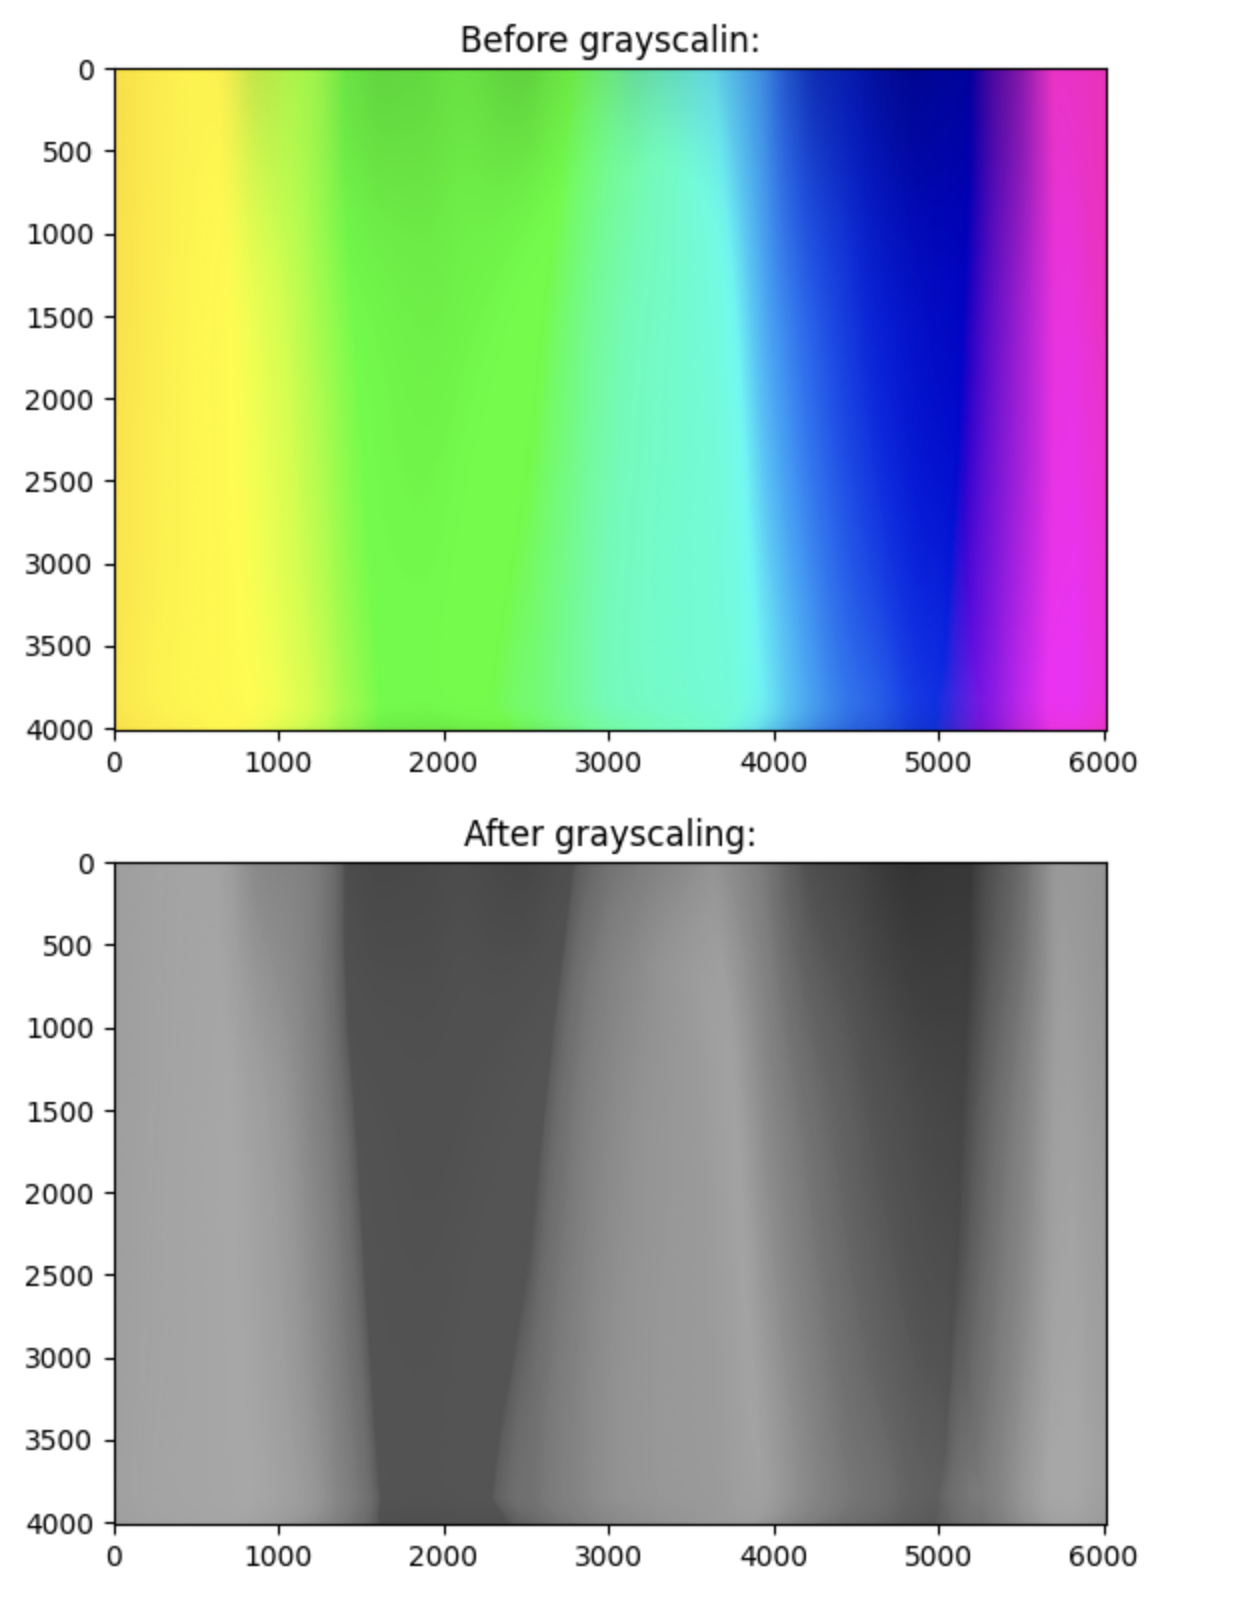
\includegraphics[width=1\linewidth]{result.png}
    \caption{Grayscaling implementation using CUDA programming}
    \label{fig:placeholder}
\end{figure}

We also, experiment different block size for different performance, and plot the graph performance of the GPU.

\begin{figure}
    \centering
    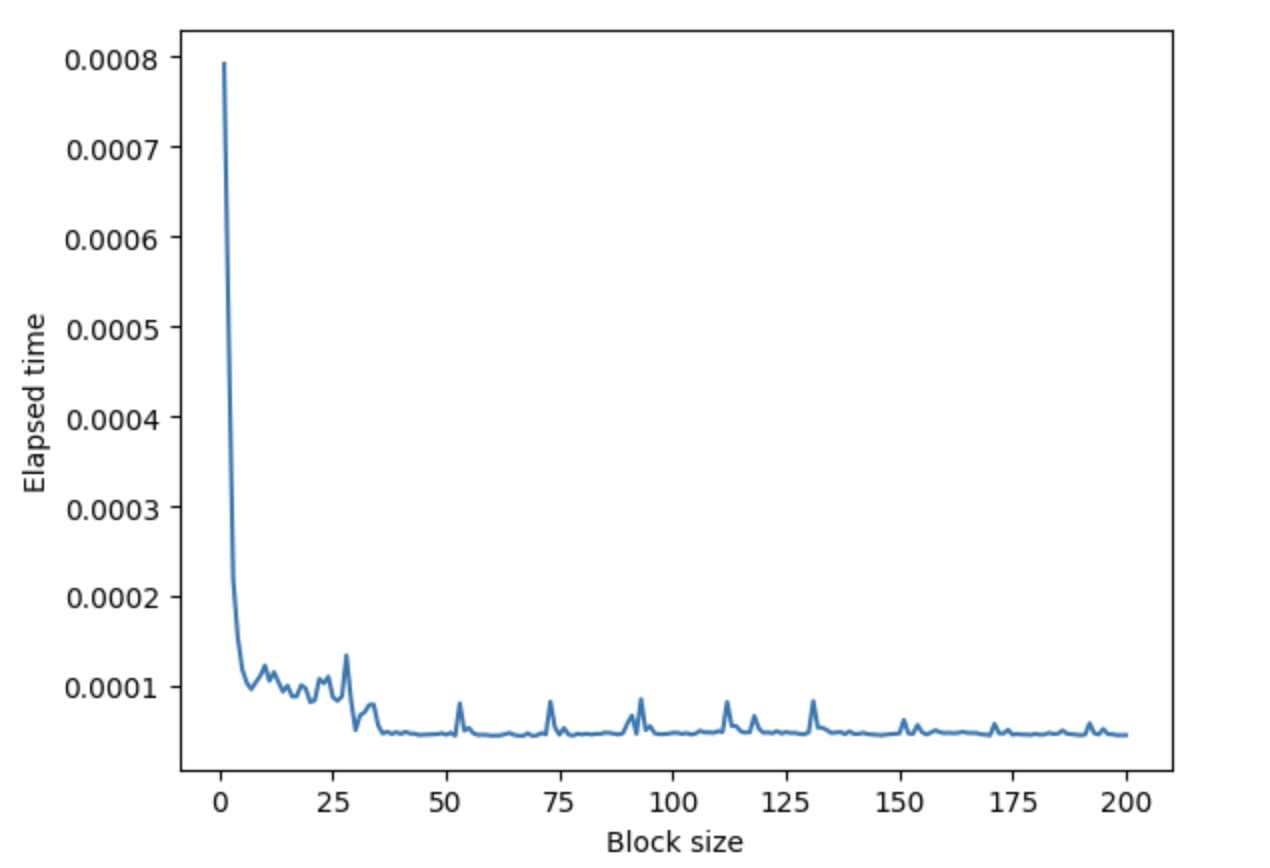
\includegraphics[width=1\linewidth]{performance.png}
    \caption{GPU performance for each different blocksize}
    \label{fig:placeholder}
\end{figure}

For reference, we refer to \href{https://colab.research.google.com/github/HamzaGbada/Numba-cuda/blob/main/Numba_CUDA.ipynb}{tutorial page on Google Colab.}

\end{document}